\section{Introducción} 

\subsection{¿Quién soy yo?}
\begin{frame}{¿Quién soy yo?}
	\begin{itemize}
		\item Ingeniero Naval y Oceánico
		\item Doctorando del programa de ingeniería aeroespacial
		\item Investigador en el canal de ensayos de la ETSIN
		\item Especializado en mecánica de fluidos computacional
		\item Desarrollador de software libre
		\begin{itemize}
			\item FreeCAD
			\item ocland
			\item SonSilentSea
			\item ...
		\end{itemize}	
	\end{itemize}
\end{frame}

\subsection{¿Qué es SonSilentSea?}
\begin{frame}{¿Qué es SonSilentSea?}
	\begin{center}
	\href{https://github.com/sanguinariojoe/sonsilentsea}{https://github.com/sanguinariojoe/sonsilentsea}
	\end{center}
	\begin{itemize}
		\item Juego de simulación naval
		\item Dedicado a Sonsoles Jiménez Caballero
		\item Software libre
		\item Desarrollado durante 3 años con \CC $\,$ y OGRE
		\item Ahora se desarrolla en Blender con Python
	\end{itemize}
	\begin{figure}
		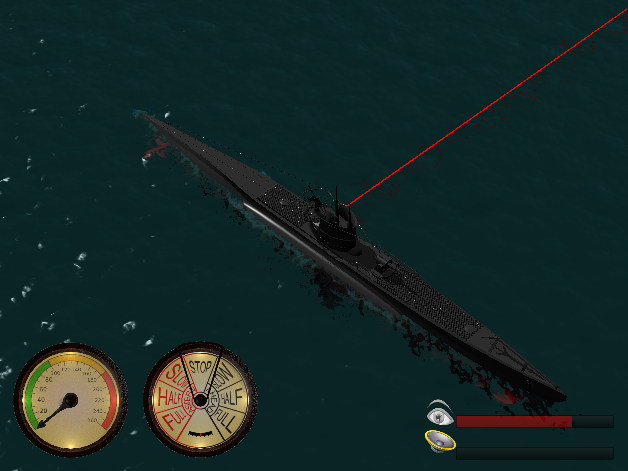
\includegraphics[scale=0.3]{screenshot0} 
	\end{figure}
\end{frame}

\subsection{¿Qué pretendo contar?}
\begin{frame}{¿Qué pretendo contar?}
	\begin{itemize}
		\item OGRE vs. Blender
		\item \textbf{\CC $\,$ vs. Python}
	\end{itemize}
	%
	\pause
	%
	O más concretamente...
	%
	\begin{itemize}
		\item Diferencias debidas a la familiaridad con el diseño,
		el lenguaje y el entorno
		% 1.- Familiaridad con el lenguaje y el entorno
		% 2.- Claridad en el diseño
		\item Diferencias debidas a una mejor integración
		% 1.- Exportacion de modelos
		%  1.b.- Zonas de suavizado
		%  1.c.- Materiales
		%  1.d.- Sistemas de referencia
		%  1.e.- Ligaduras
		% 2.- Particulas
		% 3.- Posibilidades para extender
		% 4.- Adaptacion a las necesidades
		\item Diferencias debidas a tener un framework
		% 1.- Fisicas
		% 2.- Entradas y salidas
		% 3.- Operadores logicos
		% 4.- Limitaciones
		%  4.a.- Limitacion de masa
		%  4.b.- Orden de renderizado
		\item Diferencias debidas a los estándares (ligado con la integración)
		% 1.- Modularizacion
		% 2.- CEGUI vs. bgui
		% 3.- Fragmentacion
		% 4.- Portabilidad
		\item \textbf{Diferencias debidas al lenguaje (\CC $\,$ vs. Python)}
		% 1.- Lineas de codigo
		% 2.- Errores y debugado
		% 3.- Campañas (directamente en Python frente al parser XML)
	\end{itemize}

	\vspace{0.3cm}

	\begin{center}
		Tratamos de estimar que parte se límita al cambio de lenguaje,
		pero es difícil de medir: tiempo, esfuerzo, cantidad de información...
		
		"3 años en \CC $\,$ $\rightarrow$ 2 meses en Python"
	\end{center}
	%
\end{frame}

\begin{frame}{Precedentes}
Usando algunos ejemplos de algoritmos de ordenación...

\vspace{0.5cm}
\begin{columns}
  \begin{column}{0.5\textwidth}
    \textbf{\underline{Python}}
    \begin{itemize}
        \item Bubble sort: 24 líneas
        \item Bitonic sort: 23 líneas
        \item Counting sort: 11 líneas
        \item Insertion sort: 8 líneas
        \item Merge sort: 24 líneas
        \item Heap sort: 35 líneas
        \item Radix sort: 38 líneas
    \end{itemize}
  \end{column}

  \begin{column}{0.5\textwidth}
    \textbf{\underline{\CC}}
    \begin{itemize}
        \item Bubble sort: 33 líneas (x1.4)
        \item Bitonic sort: 131 líneas (x5.7)
        \item Counting sort: 49 líneas (x4.5)
        \item Insertion sort: 9 líneas (x1.1)
        \item Merge sort: 58 líneas (x2.4)
        \item Heap sort: 53 líneas (x1.5)
        \item Radix sort: 90 líneas (x2.4)
    \end{itemize}
  \end{column}
\end{columns}

\vspace{0.5cm}
Con ésta pequeña muestra crear un algoritmo en C++ parece requerir
$2.7 \pm 1.6$ veces más líneas de código

\end{frame}

\begin{frame}{Diferencias en cuanto a características}
\begin{columns}
  \begin{column}{0.5\textwidth}
    \textbf{\underline{Blender}}
    \begin{itemize}
        \item 20 FPS en el portátil
        \item Cámara "isométrica"
        \item Sólo visión desde fuera del agua
        \item Geometría del mar simplificada por un plano
        \item Física más realista
        \item No existe necesidad de preocuparse por la atmósfera
    \end{itemize}
	\begin{figure}
		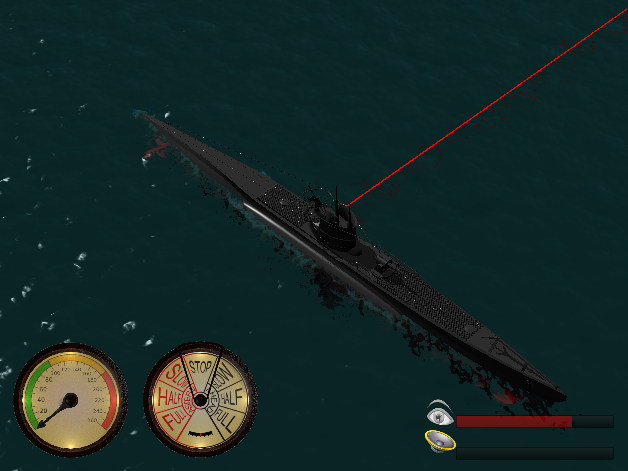
\includegraphics[scale=0.22]{screenshot0} 
	\end{figure}    
  \end{column}

  \begin{column}{0.5\textwidth}
    \textbf{\underline{OGRE}}
    \begin{itemize}
        \item Inmanejable en el portátil
        \item Cámara libre
        \item Completo entorno submarino (Hydrax)
        \item Compleja geometría del mar
        \item Física pobre
        \item Atmósfera realista (SkyX)
    \end{itemize}
	\begin{figure}
		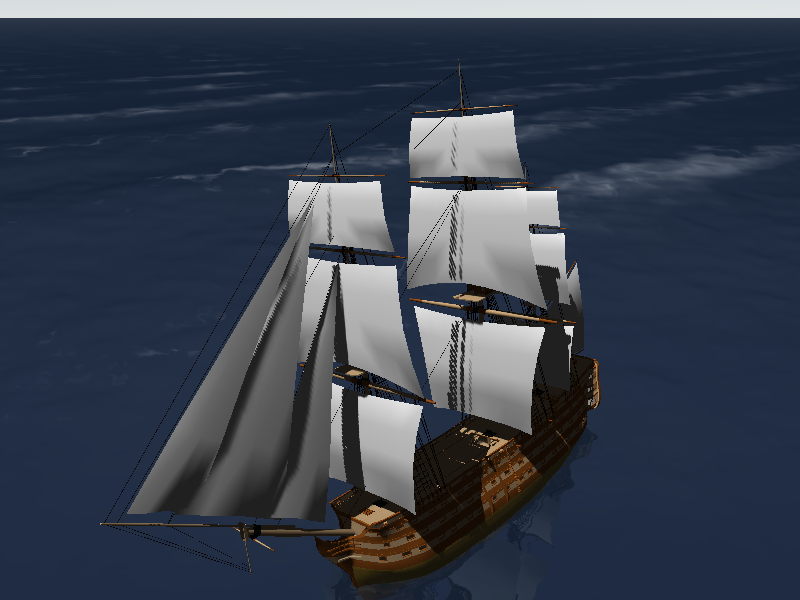
\includegraphics[scale=0.18]{old_screenshot_6} 
	\end{figure}
  \end{column}
\end{columns}
\end{frame}
